\documentclass[11pt]{scrartcl}
 
%deutsche Zeichensätze einbinden
\usepackage{ucs}
\usepackage[utf8x]{inputenc}
\usepackage[T1]{fontenc}

%Latex mitteilen, dass deutsche sprache verewendet wird
\usepackage[ngerman]{babel}

%Mathepackage der American Mathematical Society einbinden 
\usepackage{amsmath,amssymb,amstext}

%Graphic package einbinden
\usepackage{graphicx}

\usepackage{listings} 
\usepackage{xcolor}

%Autor,... festlegen
\title{Embedded Systems 1 - Dokumentation}
\author{Kevin Fritz}
\date{\today{}, Aalen}

% für Listings
\usepackage{listings}
\lstset{numbers=left, numberstyle=\tiny, numbersep=5pt, keywordstyle=\color{blue}\bfseries, stringstyle=\ttfamily,showstringspaces=false,basicstyle=\footnotesize,captionpos=b,}

%define language and add more keywords
%\lstset{language=C, %morekeywords={[2]uint8_t,uint16_t,uint32_t,uint64_t,int8_t,int16_t,int32_t,int64_t,__asm__},
%morekeywords={[3]TRISB8,ANSB8,CNIENB8,CNPUB8,CNPB8}
%}

\definecolor{bluekeywords}{rgb}{0,0,1}
\definecolor{greencomments}{rgb}{0,0.5,0}
\definecolor{redstrings}{rgb}{0.64,0.08,0.08}
\definecolor{xmlcomments}{rgb}{0.5,0.5,0.5}
\definecolor{orangestrings}{rgb}{1,0.5,0}
\definecolor{bluetypes}{rgb}{0,0.7,1}
\definecolor{types}{rgb}{0.17,0.57,0.68}

\lstset{language=C,
captionpos=b,
%numbers=left, %Nummerierung
%numberstyle=\tiny, % kleine Zeilennummern
frame=lines, % Oberhalb und unterhalb des Listings ist eine Linie
showspaces=false,
showtabs=false,
breaklines=true,
showstringspaces=false,
breakatwhitespace=true,
escapeinside={(*@}{@*)},
commentstyle=\color{xmlcomments},
morekeywords={__asm__},
morekeywords=[2]{uint8_t,uint16_t,uint32_t,uint64_t,int8_t,int16_t,int32_t,int64_t},
morekeywords={[3]TRISB8,ANSB8,CNIEB8,CNPUB8,CNPDB8, LATB8},
keywordstyle=\color{bluekeywords},
keywordstyle=[2]\color{bluetypes},
keywordstyle=[3]\color{greencomments},
stringstyle=\color{orangestrings},
basicstyle=\ttfamily\small,
}

\usepackage[
colorlinks=true,
urlcolor=blue,
linkcolor=black
]{hyperref}

\begin{document}
%Titelblatt einfügen
\maketitle
\begin{center}
	
\includegraphics[width=\textwidth]{Images/hs_aalen_logo}
\end{center}
\newpage

\tableofcontents
\newpage

\addsec{Einleitung} %addsec erhält keine nummerrierung
\label{sec:einleitung} %label erstellen für quervereise
Einleitung muss noch verfasst werden.
\newpage

\section{Getting Started}
\subsection{Aufgabenstellung}

\begin{enumerate}%Aufzählung mit Numerierung
		\item Nehmen Sie das Programm „HelloWorld2“ in Betrieb.
		\item Entfernen Sie die Verzögerungsfunktion und messen Sie die Frequenz, mit der die LED angesteuert wird. Überprüfen Sie das Ergebnis durch Analyse des generierten Assembler-Codes. Wie groß ist die Rechenleistung in MIPS?
		
		\item Erhöhen Sie die CPU-Frequenz auf den maximal möglichen Wert. Weisen Sie durch eine Messung nach, dass die CPU-Frequenz tatsächlich erhöht wurde. Wie groß ist die Rechenleistung in MIPS?
\end{enumerate}


\subsection{Lösung}
\begin{enumerate}
		\item Programm „HelloWorld2“ in Betrieb nehmen. Der Programmcode ist in Listing \ref{lst:HelloWorld2} zu sehen.
		\item Die Verzögerungsfunktion wurde auskommentiert. Der Oszi-Aufnahme aus Abbildung \ref{image:AnsteuerungsfrequenzLED} kann entnommen werden, dass die Zeitdauer um einen Port ein- bzw. auszuschalten jeweils ungefähr $5,75us$ beträgt. Daraus ergibt sich eine Frequenz von $f=\frac{1}{T}=\frac{1}{5,75us}≈174kHz$. Aus Listing \ref{lst:AssemblerToggle} geht hervor das zum Toggeln der LED 16 Assemblerbefehle benötigt werden.
		\begin{equation}
		\label{eq:MIPS}
		MIPS=\frac{16}{5,75us}*10^{-6}≈2,783  MIPS
		\end{equation}
		Die Einheit MIPS gibt an, wie viele Maschinenbefehle (Instruktionen) ein Mikroprozessor pro Sekunde ausführen kann. 1 MIPS bedeutet, er kann eine Million Maschinenbefehle pro Sekunde ausführen. MIPS ist eine ungenaue Einheit, da verschiedene Assemblerbefehle verschieden viel Zeit benötigen.
		\item Um die CPU-Frequenz auf den Maximalen Wert zu erhöhen wird die auf dem Board verbaute PLL verwendet. Die Parameter zur Konfiguration der PLL sind dem Datenblatt (Abbildung \ref{image:CPUClockingSystem}) zu entnehmen. Der Wertebereich der PLL Parameter kann Abbildung \ref{image:PLLParameter} entnommen werden. Die Parameter wurden (mit einem Excel Sheet, Abbildung \ref{image:PLLParameterExcel}) so ausgelegt, dass sich eine Taktfrequenz $F_{OSC}$ von $140 MHz$ ergibt. Aus dem Oszillator Modul (online zu finden bei mikrochip) kann eine Code-Sequenz entnommen werden wie die jeweiligen PLL-Parameter zu setzen sind. Der Ausschnitt aus dem Datenblatt wurde für unsere Zwecke angepasst (Listing \ref{lst:OscillatorSetup}).\newline		
		Nach Konfigurieren der PLL wurde wieder die Zeitdauer zum toggeln der LED gemessen ($302ns$ für 16 Assembler-Befehle), hieraus ergibt sich eine Rechenleistung von:
		\begin{equation}
		\label{eq:MIPS_140MHz}
		MIPS=\frac{16}{302ns}*10^{-6}≈52,980  MIPS
		\end{equation}
		Setzt man die ausgerechneten MIPS ins Verhältnis, kommt man zu dem Entschluss das die gemessenen Werte plausibel sind, da: $2,783*\frac{140}{7,37}≈52,867 $.
		
		
\end{enumerate}

\newpage
%\lstset{language=C}
\begin{lstlisting}[frame=htrbl, caption={Quellcode HelloWorld2}, label={lst:HelloWorld2}]
// Check for Project Settings
#ifndef __dsPIC33EP512MU810__
#error "Wrong Controller"
#endif
#include <xc.h>    //Include appropriate controller specific headers
#include <stdint.h>//Standard typedefs
// Oscillator Configuration
_FOSCSEL(FNOSC_FRC); //Initial Oscillator:  Internal Fast RC
_FOSC(POSCMD_NONE);  //Primary Oscillator disabled (not used)

/* Substitute for stdlib.h */
#define	EXIT_SUCCESS	0
#define	EXIT_FAILURE	1

/* Hardware  */
#define _LED200 LATBbits.LATB8

void delay_ms(uint16_t u16milliseconds){
	uint16_t ui16_i=0;
	while(u16milliseconds){
		for (ui16_i=0;ui16_i<331;ui16_i++){//1 ms delay
			__asm__ volatile("nop \n\t"
			"nop \n\t"
			"nop \n\t");
		}//for
	u16milliseconds--;
	}//while
}
int main() {
/* Port Configurations */ // DS70616G-page 209
// ODCB (open drain config) unimplemented (DS70616G, Table 4-56)
ANSELBbits.ANSB8=0;     //Digital I/O
CNENBbits.CNIEB8=0;     //Disable change notification interrupt
CNPUBbits.CNPUB8=0;     //Disable weak pullup
CNPDBbits.CNPDB8=0;     //Disable weak pulldown
TRISBbits.TRISB8=0;     //Pin B8: Digital Output
LATBbits.LATB8=0;       //Pin B8: Low
/* Endless Loop */
while(1){
	/* LATBbits.LATB8 = !(LATBbits.LATB8); //Toggle Pin B8 */
	_LED200=!_LED200; //Toggle LED
	delay_ms(500);
}//while
return (EXIT_SUCCESS);  //never reached
} //main()
\end{lstlisting}
\newpage
\begin{figure}
	\centering
	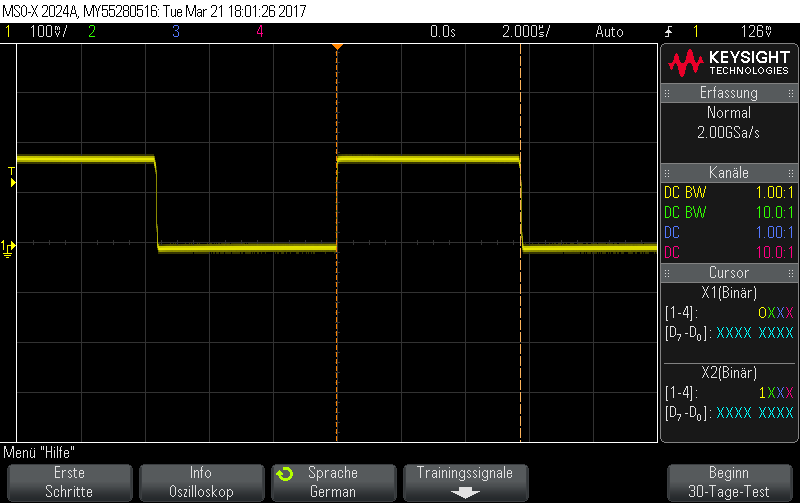
\includegraphics[width=\textwidth]{Images/1_1_MIPS}
	\caption[AnsteuerungsfrequenzLED]{Ansteuerungsfrequenz der LED}
	\label{image:AnsteuerungsfrequenzLED}
\end{figure}


\begin{lstlisting}[frame=htrbl, caption={Assembler Befehle zum toggeln}, label={lst:AssemblerToggle}]
//while(1){
// _LED200=!_LED200; //Toggle LED
00033E  8070A1     MOV LATB, W1
000340  201000     MOV #0x100, W0
000342  608000     AND W1, W0, W0
000344  A7F000     BTSC W0, #15
000346  EA0000     NEG W0, W0
000348  E90000     DEC W0, W0
00034A  DE004F     LSR W0, #15, W0
00034C  784000     MOV.B W0, W0
00034E  FB8000     ZE W0, W0
000350  600061     AND W0, #0x1, W0
000352  DD0048     SL W0, #8, W0
000354  8070A1     MOV LATB, W1
000356  A18001     BCLR W1, #8
000358  700001     IOR W0, W1, W0
00035A  8870A0     MOV W0, LATB
//}//while
00035C  37FFF0     BRA 0x33E
//return (EXIT_SUCCESS);  //never reached
//} //main()
\end{lstlisting}	
\newpage

\begin{figure}
	\centering
	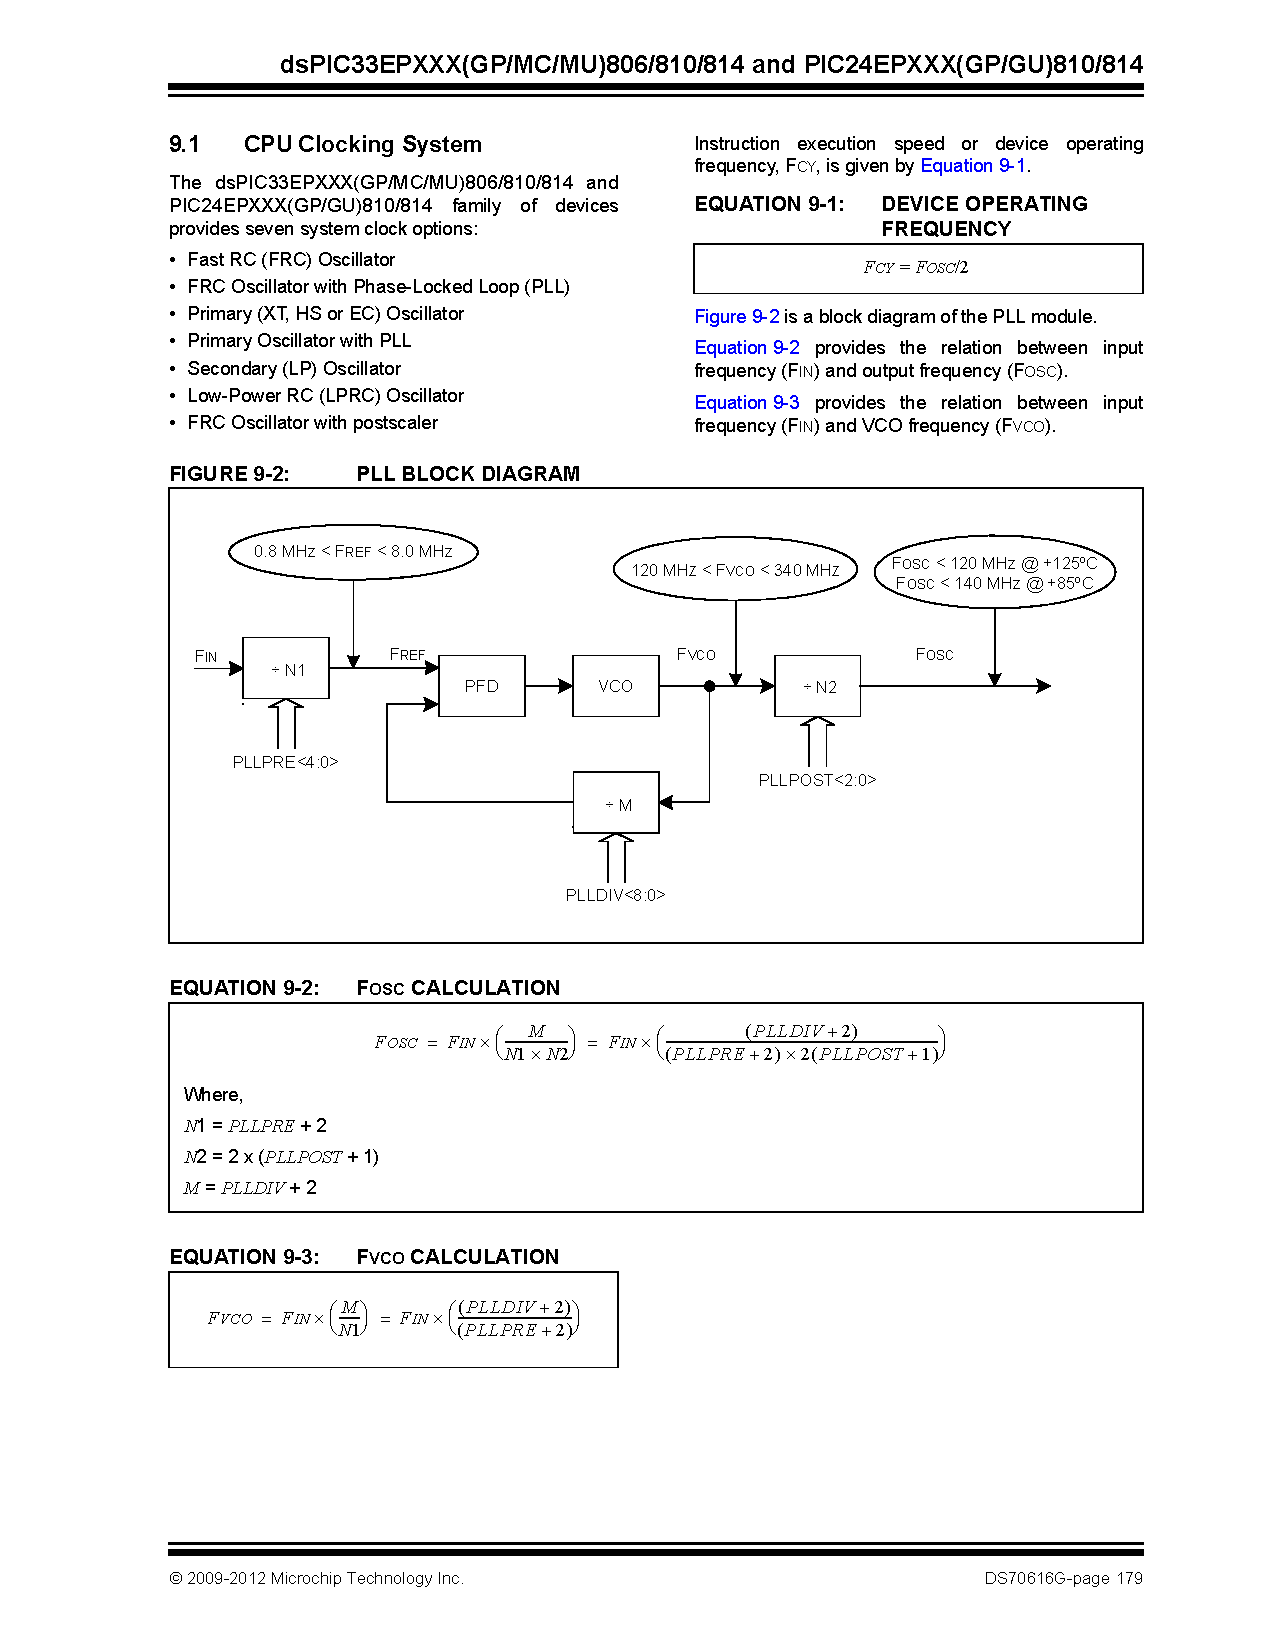
\includegraphics[width=\textwidth]{Images/CPUClockingSystem}
	\caption[CPU Blocking System]{CPU Clocking System mit PLL Block Diagramm}
	\label{image:CPUClockingSystem}
\end{figure}

\begin{figure}
	\centering
	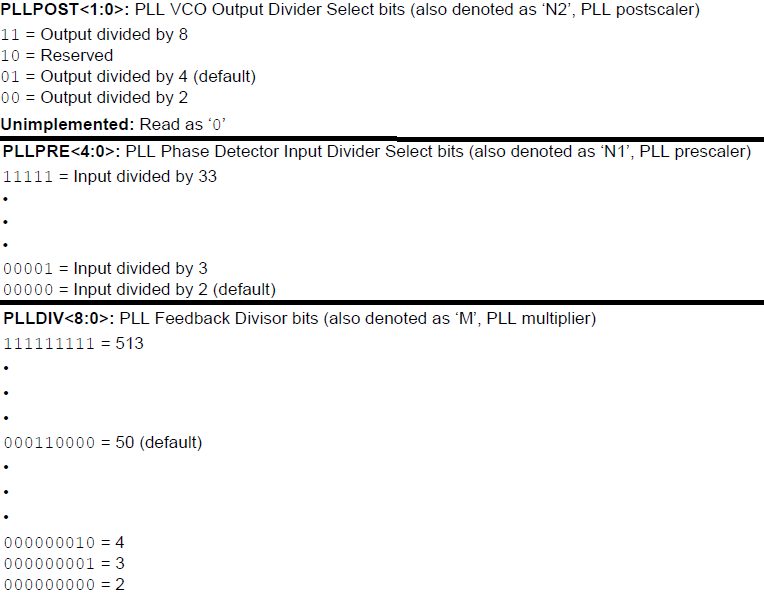
\includegraphics[width=\textwidth]{Images/PLLParameter}
	\caption[Wertebereich der PLL Parameter]{Wertebereich der PLL Parameter}
	\label{image:PLLParameter}
\end{figure}

\begin{figure}
	\centering
	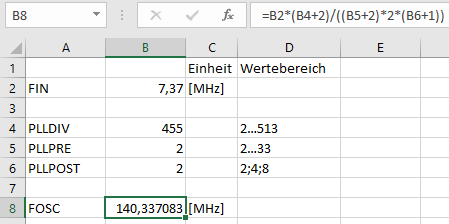
\includegraphics[width=0.95\textwidth]{Images/PLLParameterExcel}
	\caption[Berechnung der PLL Parameter in Excel]{PLL Parameter Excel}
	\label{image:PLLParameterExcel}
\end{figure}

\newpage
\begin{lstlisting}[frame=htrbl, caption={Code Example for Using PLL with 7.37 MHz Internal FRC}, label={lst:OscillatorSetup}]
// Select Internal FRC at POR
_FOSCSEL(FNOSC_PRIPLL); //Initial Oscillator: Primary Oscillator (XT, HS, EC) with PLL
_FOSC(POSCMD_HS);  //HS Crystal Oscillator Mode

int main()
{
// Configure PLL prescaler, PLL postscaler, PLL divisor
PLLFBD=455; // PLLDIV
CLKDIVbits.PLLPOST=2;
CLKDIVbits.PLLPRE=2;

// Wait for PLL to lock
while (OSCCONbits.LOCK!= 1);


while(1)
{
//endless loop
}

return 1; //never reached
}
\end{lstlisting}

\newpage

\section{Rechenleistung}
\subsection{Aufgabenstellung}

\begin{enumerate}%Aufzählung mit Numerierung
		\item Ermitteln Sie die durchschnittliche Laufzeit einschließlich Streuung arithmetischer Grundoperationen für verschiedene vom XC-16-Compiler unterstützten Datentypen. Wie erklären Sie die Unterschiede?
		\item Berechnen Sie die ersten 10 Primzahlen, die größer als 1.000.000 (1E6) sind. Implementieren Sie denselben Algorithmus auf einem PC und vergleichen Sie die Rechenzeiten.
		
\end{enumerate}

\subsection{Lösung}
\begin{enumerate}
		\item 
		Der Programmcode wird so umgeändert wie in Listening  \ref{lst:Rechenleistung} zu sehen. Zuerst wird mit dem Oszi nur die Zeit gemessen wie lange eine LED aus ist (ohne Rechenoperation, $29,1 ns$). Anschließend kann man mit dem Oszi messen wie lange eine Grundoperation (mit Zufallszahlen) inklusiv LED ein/ausschalten benötigt. Die folgende Auflistung beinhaltet nur die Zeitdauer für die jeweilige Rechenoperation (ohne LED ein/aus).\newline
\begin{tabular}{|c|c|c|c|c|c|c|}
	\hline 
	Datentyp & Operation & Zeitdauer &  & Datentyp & Operation & Zeitdauer \\
	\hline
	
	\hline
	uint8\_t 	& + & 43,7 ns &  		& int8\_t 		& + & 57,4 ns \\ 
	\hline 
				& - & 58,1 ns &  		&  				& - & 57,4 ns \\ 
	\hline 
				& * & 72,1 ns &  		&  				& * & 71,9 ns \\ 
	\hline 
				& / & 72,5 ns &  		&  				& / & 343,9 ns \\ 
	\hline 

	%&  &  &  &  &  &  \\ %empty Line 
	\hline 
	uint16\_t 	& + & 43,4 ns &  		& int16\_t 		& + & 43,3 ns \\ 
	\hline 
				& - & 43,5 ns &  		&  				& - & 43,4 ns \\ 
	\hline 
				& * & 86,2 ns &  		&  				& * & 87,4 ns \\ 
	\hline 
				& / & 330,9 ns &  		&  				& / & 329,9 ns \\ 
	\hline

	%&  &  &  &  &  &  \\ %empty Line 
	\hline 
	uint32\_t 	& + & 115,4 ns &  		& int32\_t 		& + & 142,9 ns \\ 
	\hline 
				& - & 114,9 ns &  		&  				& - & 112,9 ns \\ 
	\hline 
				& * & 245,9 ns &  		&  				& * & 230,9 ns \\ 
	\hline 
				& / & 7,559 us &  		&  				& / & 7,95 us \\ 
	\hline

	%&  &  &  &  &  &  \\ %empty Line 
	\hline 
	uint64\_t 	& + &  &  		& int64\_t 		& + & 254,9 ns \\ 
	\hline 
				& - &  &  		&  				& - & 226,9 ns \\ 
	\hline 
				& * &  &  		&  				& * & 1,5 us \\ 
	\hline 
				& / &  &  		&  				& / & 131 us \\ 
	\hline

	%&  &  &  &  &  &  \\ %empty Line 
	\hline 
	float 	& + &  &  				& long double 		& + &  \\ 
	\hline 
			& - &  &  		&  							& - &  \\ 
	\hline 
			& * &  &  		&  							& * &  \\ 
	\hline 
			& / &  &  		&  							& / &  \\ 
	\hline  
\end{tabular} 			
\newpage

		\item Der geforderte Algorithmus ist in Listening \ref{lst:Primzahlen} abgebildet. Bei dem verfügbaren Computer (Intel Core i7 2.6GHz, 16GB RAM, 64Bit Windows 10) ergab sich eine Laufzeit von ungefähr $5 us$. (Gemessen mit CodeBlocks, $50 s$ für $10^7$ Durchläufe)
		
		Die Laufzeit des selben Programms (angepasst auf die Hardware) benötigte auf dem Mikrocontroller Board $47,8 ms$. Der Code hierzu ist in Listing \ref{lst:PrimzahlenuC} abgebildet.
		
		Damit ist der Computer ca 10.000 mal schneller als der µC.
		 ($\frac{47,8 ms}{5 us} = 9560 $, Abbildung \ref{image:scopePrimzahlen}).
\end{enumerate}

\begin{figure}[h]
	\centering
	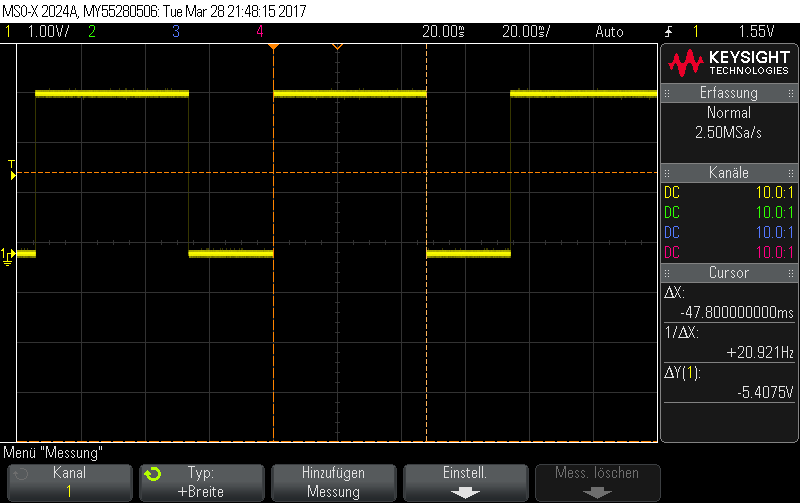
\includegraphics[width=\textwidth]{Images/scope_primzahlen}
	\caption[Laufzeit der Primzahlenberechnung]{Laufzeit der Primzahlenberechnung}
	\label{image:scopePrimzahlen}
\end{figure}

\newpage
\begin{lstlisting}[frame=htrbl, caption={Bestimmen der Rechenleistung}, label={lst:Rechenleistung}]
/* Endless Loop */
while(1){
_LED200=0;
ui8Var1 *= ui8Var2;
_LED200=1;
}//while
\end{lstlisting}

\begin{lstlisting}[frame=htrbl, caption={Algorithmus zur Berechnung der ersten 100 Primzahlen größer als 1E6}, label={lst:Primzahlen}]
#include<stdint.h>
#include<stdlib.h>
#include<math.h>

uint8_t isPrim(uint32_t ui32Number);

int main()
{
	uint32_t ui32Number= 1e6;  //start value
	uint16_t ui8PrimeCounter=0; //counts the number of calculated prime numbers
	const uint16_t ui8PrimMax=100;

	for(; ui8PrimeCounter<ui8PrimMax; ui32Number++)
		if(isPrim(ui32Number)) //check if the number is prime
		{
		//printf("%d\t%d\n",ui8PrimeCounter,ui32Number);
		ui8PrimeCounter++; //increase PrimeCounter, if the number is prime
		}
	return 0;
}
uint8_t isPrim(uint32_t ui32Number){
	uint32_t ui32Divider;
	uint32_t ui32SqrtNumber =((uint32_t) sqrt((double)(ui32Number)))+1;
	for(ui32Divider=2; ui32Divider<ui32SqrtNumber; ui32Divider++)
	{
		if((ui32Number%ui32Divider) == 0)
		{
			return 0; //uiNumber32 isn't a prime number
		}
	}
	return 1; //ui32Number is a Prime Number
}
\end{lstlisting}

\begin{lstlisting}[frame=htrbl, caption={Algorithmus zur Berechnung der ersten 100 Primzahlen größer als 1E6 auf dem uC}, label={lst:PrimzahlenuC}]
int main() {    //scope_25 47,8ms
	
	PLLFBD = 418;
	CLKDIVbits.PLLPOST = 2;
	CLKDIVbits.PLLPRE = 2;
	
	/* Port Configurations */
	// DS70616G-page 209
	// ODCB (open drain config) unimplemented (DS70616G, Table 4-56)
	ANSELBbits.ANSB8=0;     //Digital I/O
	CNENBbits.CNIEB8=0;     //Disable change notification interrupt
	CNPUBbits.CNPUB8=0;     //Disable weak pullup
	CNPDBbits.CNPDB8=0;     //Disable weak pulldown
	TRISBbits.TRISB8=0;     //Pin B8: Digital Output
	LATBbits.LATB8=0;       //Pin B8: Low
	_LED200 = 1;
	//uint32_t    ui32Var1=2;
	//uint32_t    ui32Var2=2;
	//uint32_t    ui32Var3=2;
	while (OSCCONbits.LOCK!= 1);
	/* Endless Loop */
	
	uint32_t ui32Number= 1000000;     //start value
	uint16_t ui8PrimeCounter=0;       //counts the number of calculated prime numbers
	const uint16_t ui8PrimMax=10;
	
	while(1){
		
		_LED200=1;      //hard on/off 28,5ns  scope_15
		
		ui32Number= 1000000;     //start value
		ui8PrimeCounter=0;       //counts the number of calculated prime numbers
		//ui8PrimMax=10;
		
		for(; ui8PrimeCounter<ui8PrimMax; ui32Number++)
		if(isPrim(ui32Number)) //check if the number is prime
		{
			//printf("%d\t%d\n",ui8PrimeCounter,ui32Number);
			ui8PrimeCounter++; //increase PrimeCounter, if the number is prime
		}
		
		_LED200=0; 
		delay_ms(500);
		
	}//while
	
	return (EXIT_SUCCESS);  //never reached
} //main()

uint8_t isPrim(uint32_t ui32Number){
	
	if(ui32Number==0 || ui32Number==1)
	return 0;
	
	
	if((ui32Number%2)==0)
	{
		if(ui32Number==2)
		{
			return 1;
		}
		else
		{
			return 0;
		}
	}
	uint32_t ui32Divider;
	uint32_t ui32SqrtNumber =((uint32_t) sqrt((long double)(ui32Number)))+1;
	
	for(ui32Divider=3; ui32Divider<ui32SqrtNumber; ui32Divider+=2)
	{
		if((ui32Number%ui32Divider) == 0) //check if ui32Divider is a in whole divider of ui32Number
		{
			return 0; //uiNumber32 isn't a prime number
		}
	}
	return 1; //ui32Number is a Prime Number
}
\end{lstlisting}
\newpage

\section{IO-Bibliothek}
\subsection{Aufgabenstellung}
Die populäre Arduino-Plattform (\url{https://www.arduino.cc/en/Reference/}) 
kapselt die Pinkonfiguration und -ansteuerung mit folgenden Funktionen:
\begin{itemize}
\item pinMode()
\item digitalRead()
\item digitalWrite()
\end{itemize}
Übertragen Sie dieses Konzept auf das EDA-Board. Anwendungsbeispiele:
\begin{itemize}
\item pinMode(SW1, IPUT\_PULLUP)
\end{itemize}
soll den Pin, an den SW1 angeschlossen ist, als digitalen Eingang konfigurieren und den Pullup-Widerstand einschalten.
\begin{itemize}
	\item digitalWrite(LED203, HIGH)
\end{itemize}
soll an dem Pin, an den LED203 angeschlossen ist,
einen High-Pegel ausgeben.
Verwenden Sie die Bezeichner aus dem Schaltplan.
Modularisieren Sie Ihre Software, verwenden Sie dazu die Dateinamen \textit{edaPIC33Hardware.h} und \textit{edaPIC33Hardware.c}.\newline \newline
Dokumentieren Sie die Funktionen mit Doxygen.\newline \newline
Messen Sie die Zeit, die zur Ansteuerung eines Ausgangspins mit den IO-Bibliotheksfunktionen notwendig ist
und vergleichen Sie diese mit einem direkten Schreiben in die entsprechenden Hardwareregister.

\subsection{Lösung}
Alle Device-Pins (ausgenommen VDD, VSS, MCLR and OSC1/CLKI) sind aufgeteilt auf die Ports für Peripheriegeräte und parallel I/O Ports. Alle I/O Ports sind Schmitt-Trigger Input (verbesserte Störungsunempfindlichkeit / Rauschempfindlichkeit).\newline
Alle Port Pins besitzen acht Register, durch diese Register lässt sich der I/O Port wie in Tabelle \ref{tab:ioports} dargestellt konfigurieren. Die Register Maps sind in Abbildung \ref{image:PORTA}-\ref{image:PORTG} dargestellt.\newline\newline
Ein Beispiel wie auf die einzelnen Register Bits zugegriffen werden kann und wie ein Port konfiguriert werden kann ist in Listing \ref{lst:confregport} zu sehen.\newline\newline
Die relevanten Auszüge aus dem Datenblatt sind in den Abbildungen \ref{image:page207}-\ref{image:page209} abgebildet.\newline\newline
Es wurde die Bibliothek mit den Dateien \textit{edaPIC33Hardware.h} und \textit{edaPIC33Hardware.c} erstellt. Die Funktion wurde mit Doxygen dokumentiert (TODO Anhang...).

\newpage
\begin{table}
\begin{tabular}{|l|l|}
	\hline 
	\textbf{Register Bit} & \textbf{Function}\\ 
	\hline
	TRISx 	&determines whether the pin is an input 	or an output\\
			&0:=output, 1:=input\\
			&default: all port pins are defined as inputs after a reset\\
	\hline 
	PORTx 	&read reads the port, write writes the latch \\ 
	\hline 
	LATx 	&read reads the latch, write writes the latch \\ 
	\hline 
	ODCx 	&configures pin for digital or open-drain output \\
			&0:=digital output, 1:=open drain output\\
	\hline 
	CNENx 	&enables change notification (CN) interrupts\\
			&0:=interrupts disabled, 1:=interrupts enabled\\
	\hline 
	CNPUx 	&enables weak pullup\\
			&0:=pullup disabled, 1:=pullup enabled\\  
	\hline 
	CNPDx 	&enables weak pulldown\\
			&0:=pulldown disabled, 1:=pulldown enabled\\  
	\hline 
	ANSELx 	&controls the operation of the analog port pins\\
			&0:=port operates as digital I/O port\\
			&1:=port operates as analog I/O port\\
	\hline
	note 	&Any bit and its associated data and control registers that are not\\
			&valid for a particular device is disabled. This means the correspon\\
			&-ding LATx and TRISx registers and the port pin are read as zeros.\\
	\hline
	note	&The open-drain feature allows the generation of outputs higher\\
			&than VDD (e.g., 5V on a 5V tolerant pin) by using external pull-up\\
			&resistors. The maximum open-drain voltage allowed is the same as \\
			&the maximum VIH specification for that pin.\\
	\hline
	note	&Pull-ups and pull-downs on change notification (CN) pins should\\
			&be disabled when the port pin is configured as a digital output.\\
	\hline
\end{tabular}
\caption{Konfigurationsmöglichkeiten der I/O Ports}
\label{tab:ioports}
\end{table}

\begin{lstlisting}[frame=htrbl, caption={Konfigurieren des Ports RB8 als Digitaler Input mit Pullup Widerstand}, label={lst:confregport}]
//configure RB8 as digit input with pullup
TRISBbits.TRISB8=1;     //configure as input
ANSELBbits.ANSB8=0;     //configure as digital
CNENBbits.CNIEB8=0;     //disable change notification interrupt
CNPUBbits.CNPUB8=1;     //enable weak pullup
CNPDBbits.CNPDB8=0;     //disable weak pulldown
\end{lstlisting}




\newpage

\section{Mitschrift aus Vorlesung}
\subsection{Vorlesung 04.04.2017 - IO-Bibliothek}

\begin{itemize}%Aufzählung mit Numerierung
		\item jeder uC is universell aufgebaut und muss für jeden Fall individuell konfiguriert werden
		\item kleine Bibliothek zum anpassen der IO-Ports ist praktisch
		\item Lese und Schreib Funktionalität soll realisiert werden
		\item Datenblatt Figure 11-1 -> Pins müssen über Treiber realisiert werden, Schmitt-Trigger ist enthalten
		\item Pegel um Treiber zu aktivieren? nachlesen Schaltbild könnte falsch sein
		\item Lesezugriff über Port, Schreibezugriff über Latch
		\item Erkenntnis: Lesen des Datenblattes liefert Aufschluss wie die Pins zu beschalten sind. 
		
\end{itemize}

\subsection{Lösung}
\begin{enumerate}
		\item Lösungsansatz 1
		\item Lösungsansatz 2
		\item Lösungsansatz 3
		\item Lösungsansatz 4
\end{enumerate}


%Beispiel für Quellcode Listening
\begin{lstlisting}[frame=htrbl, caption={Listening Bezeichnung}, label={lst:Referenzname}]
//Quellcode
\end{lstlisting}


\newpage

\addsec{Anhang} %addsec erhält keine nummerrierung
\label{sec:anhang} %label erstellen für quervereise

\begin{figure}[h!]
	\centering
	\subfigure[Register A]{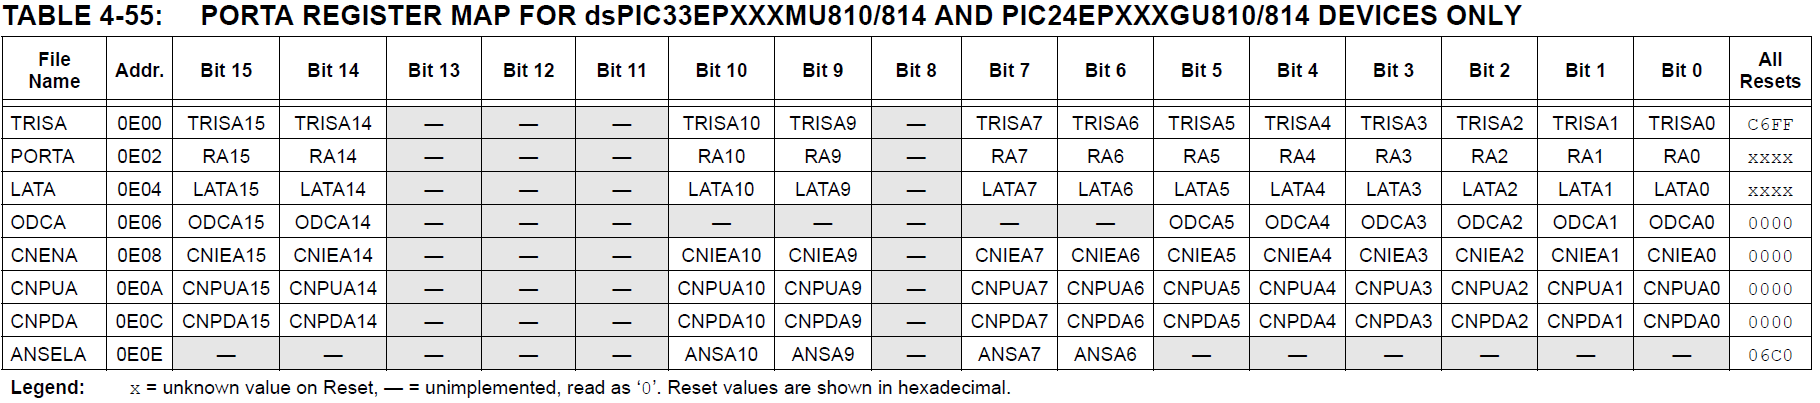
\includegraphics[width=0.8\textwidth]{Images/PORTA}} 
	\subfigure[Register B]{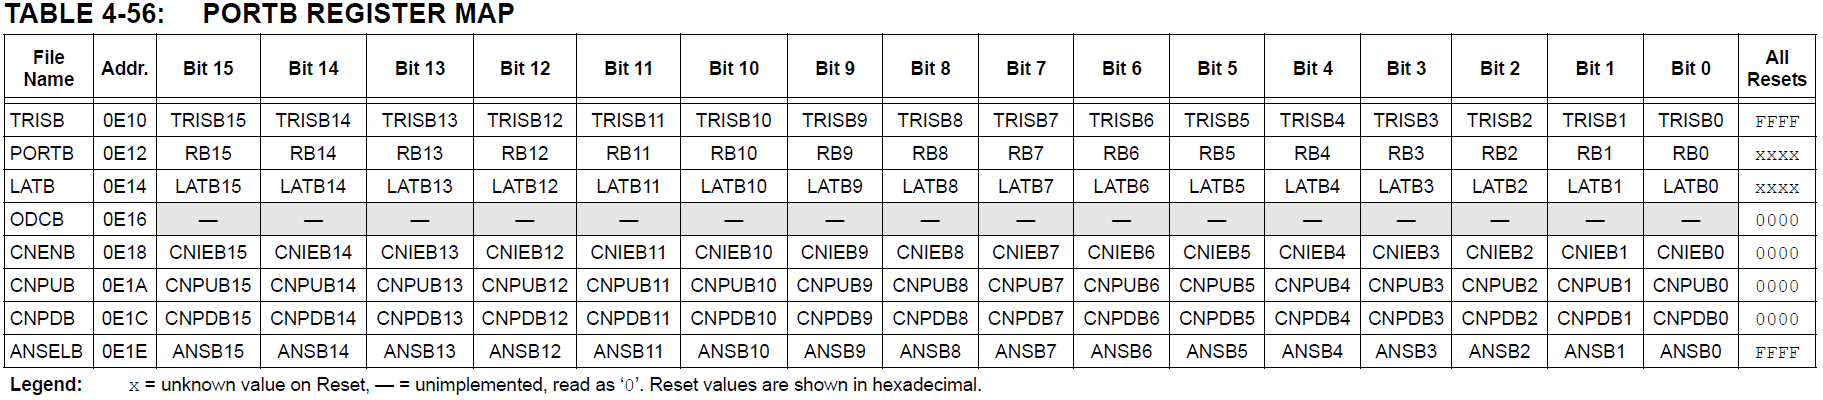
\includegraphics[width=0.8\textwidth]{Images/PORTB}} 
	\subfigure[Register C]{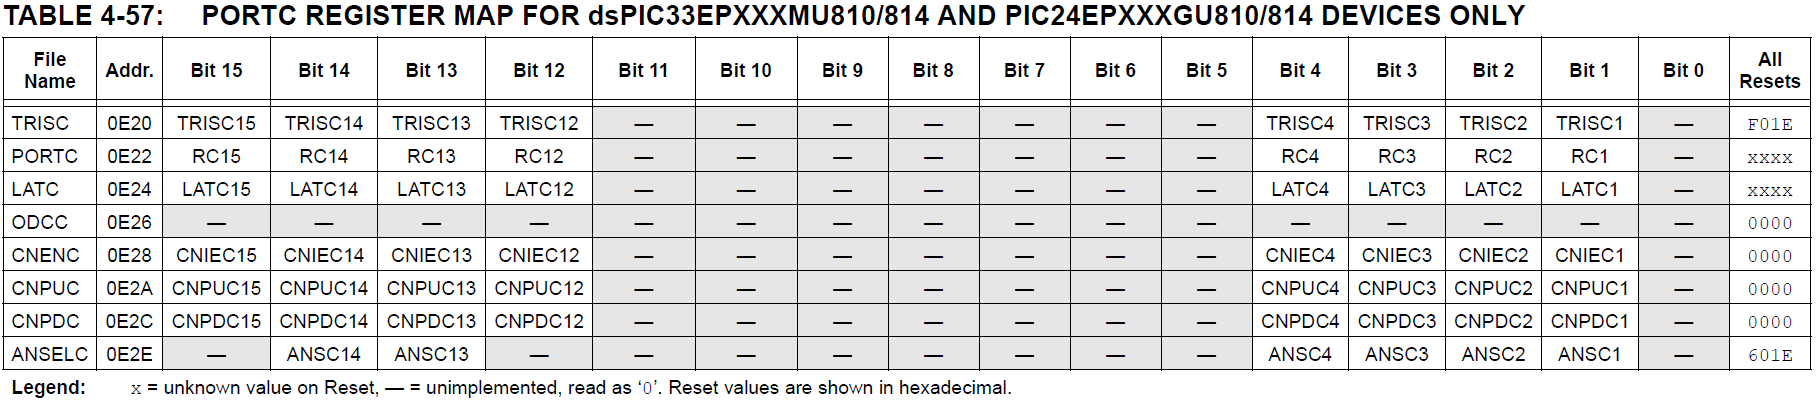
\includegraphics[width=0.8\textwidth]{Images/PORTC}} 
	\subfigure[Register D]{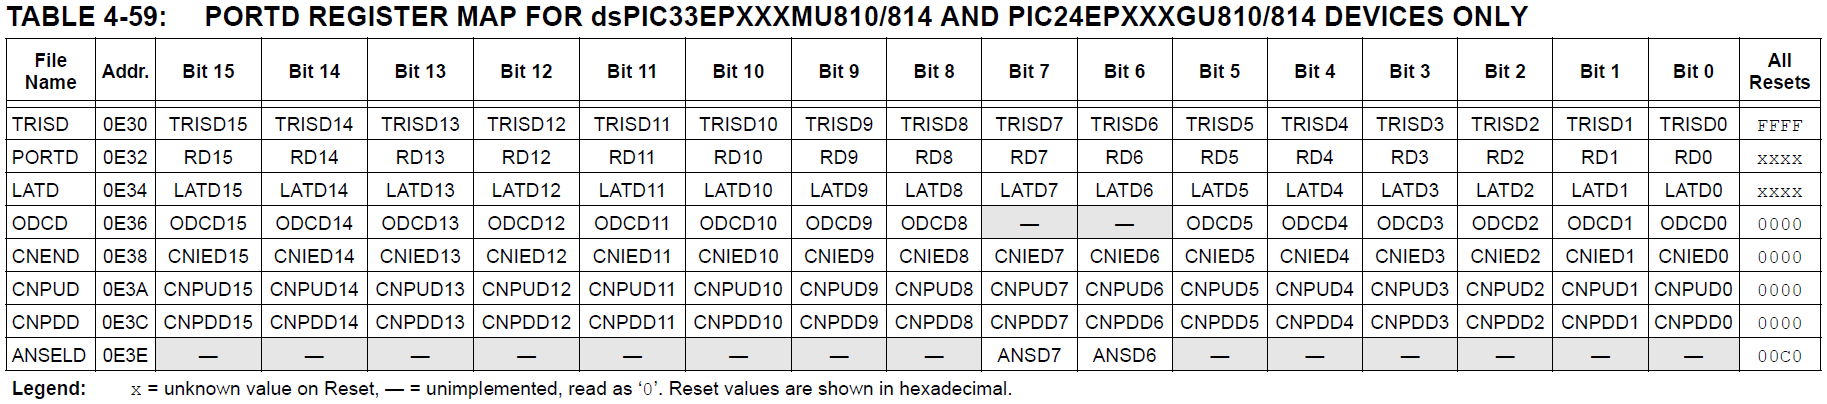
\includegraphics[width=0.8\textwidth]{Images/PORTD}} 
	\subfigure[Register E]{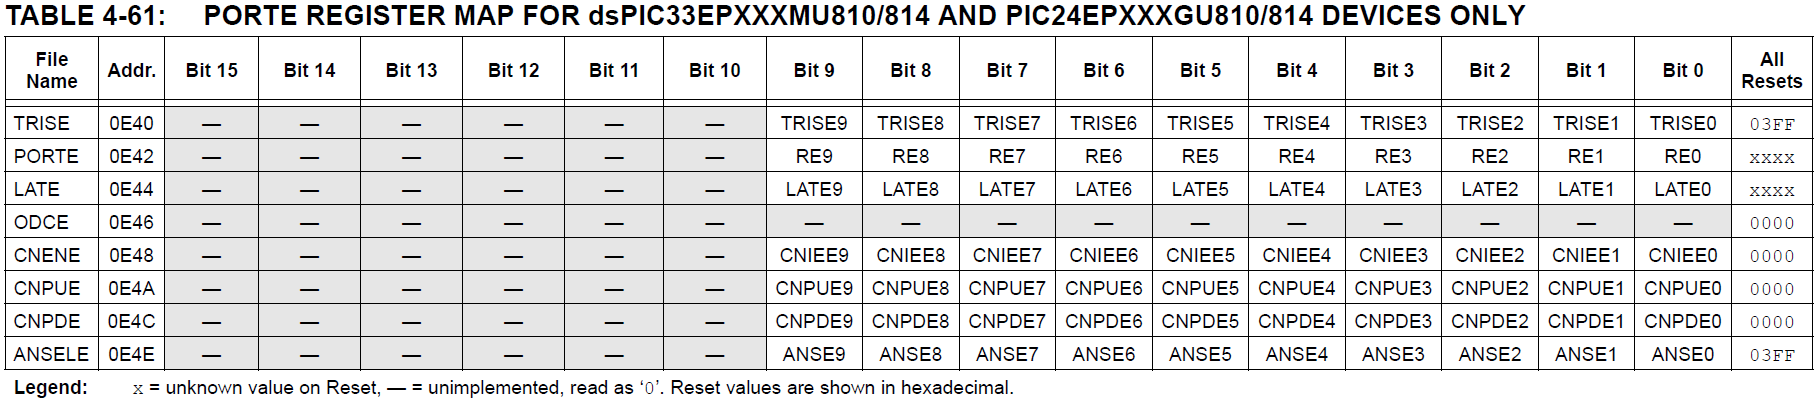
\includegraphics[width=0.8\textwidth]{Images/PORTE}} 
	\subfigure[Register F]{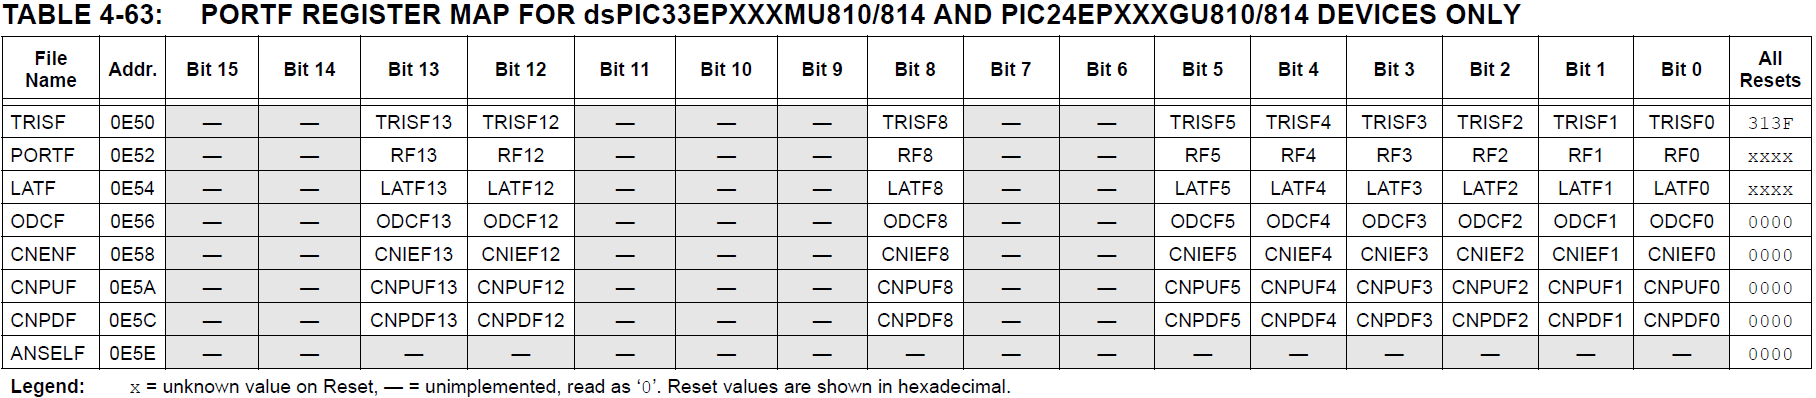
\includegraphics[width=0.8\textwidth]{Images/PORTF}}
	\subfigure[Register G]{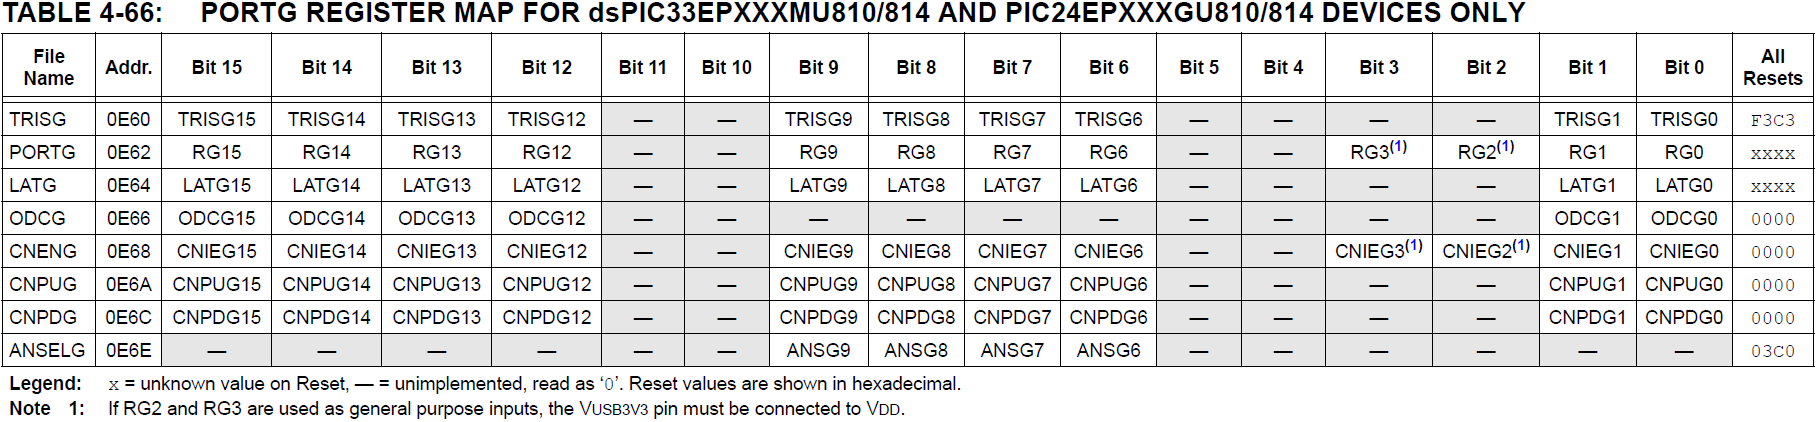
\includegraphics[width=0.8\textwidth]{Images/PORTG}}   
	\caption{PORTA-G Register Map}
	\label{image:PortMap}
\end{figure}

%
%\begin{figure}[h]
%	\centering
%	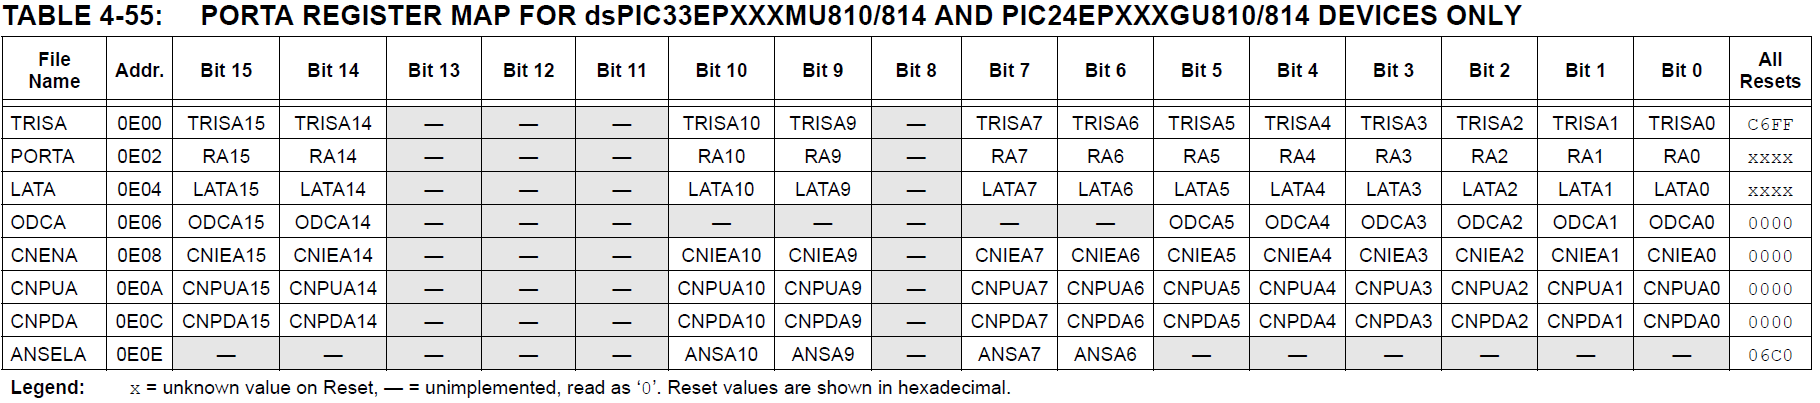
\includegraphics[width=\textwidth]{Images/PORTA}
%	\caption[PORTA Register Map]{PORTA Register Map}
%	\label{image:PORTA}
%\end{figure}
%
%\begin{figure}[h]
%	\centering
%	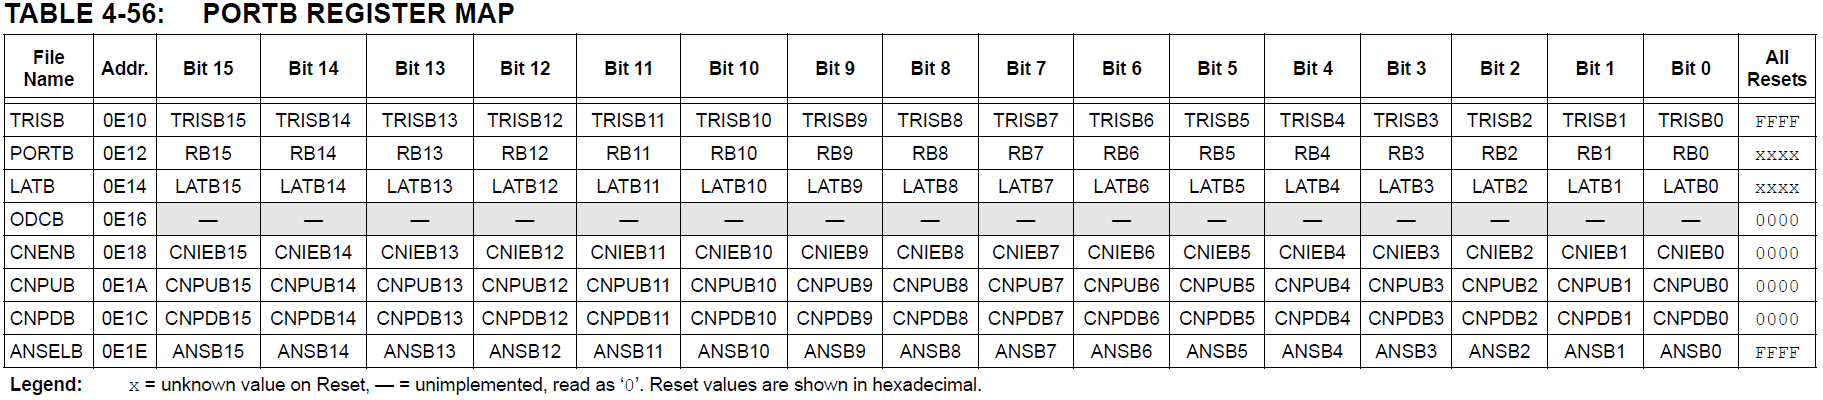
\includegraphics[width=\textwidth]{Images/PORTB}
%	\caption[PORTB Register Map]{PORTB Register Map}
%	\label{image:PORTB}
%\end{figure}
%
%\begin{figure}[h]
%	\centering
%	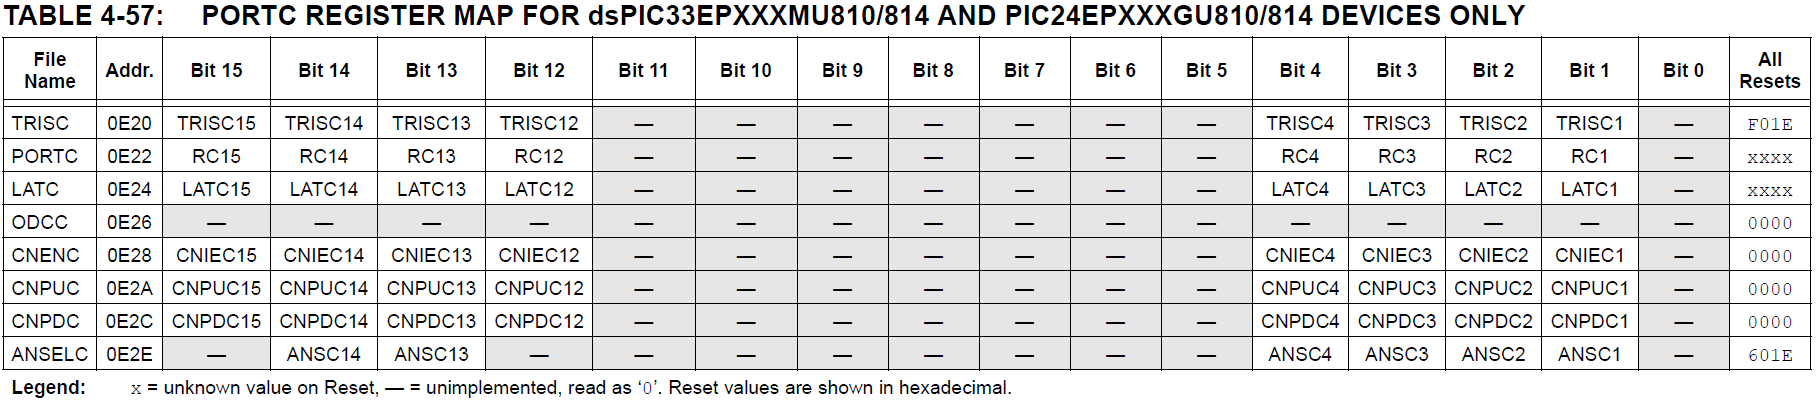
\includegraphics[width=\textwidth]{Images/PORTC}
%	\caption[PORTC Register Map]{PORTC Register Map}
%	\label{image:PORTC}
%\end{figure}
%
%\begin{figure}[h]
%	\centering
%	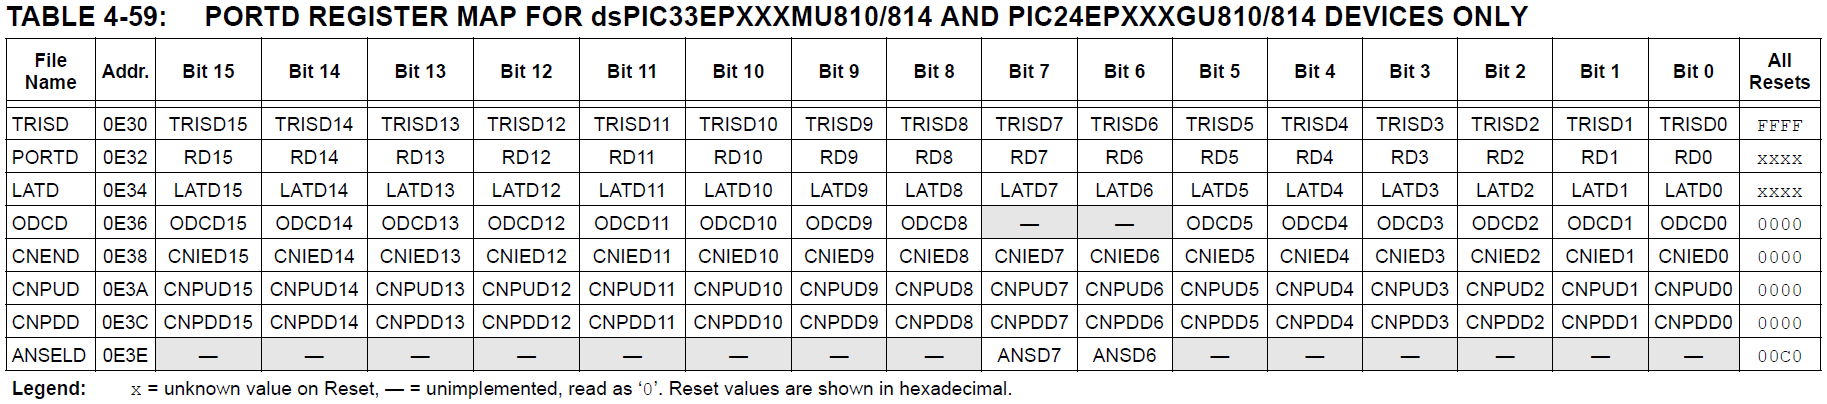
\includegraphics[width=\textwidth]{Images/PORTD}
%	\caption[PORTD Register Map]{PORTD Register Map}
%	\label{image:PORTD}
%\end{figure}
%
%\begin{figure}[!h]
%	\centering
%	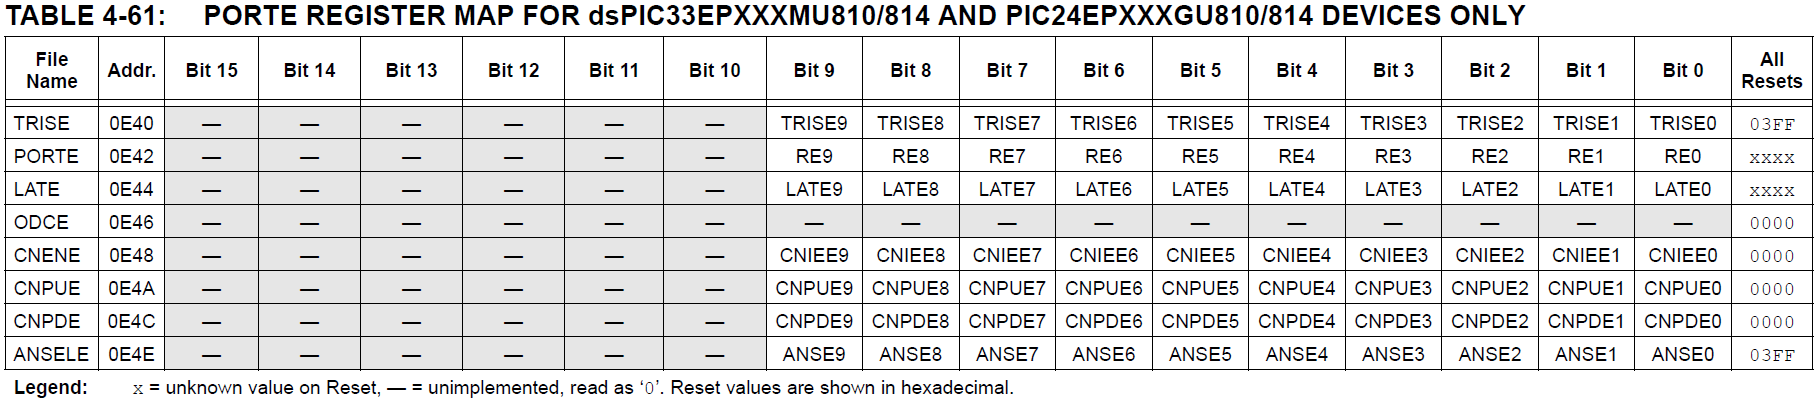
\includegraphics[width=\textwidth]{Images/PORTE}
%	\caption[PORTE Register Map]{PORTE Register Map}
%	\label{image:PORTE}
%\end{figure}
%
%\begin{figure}[!h]
%	\centering
%	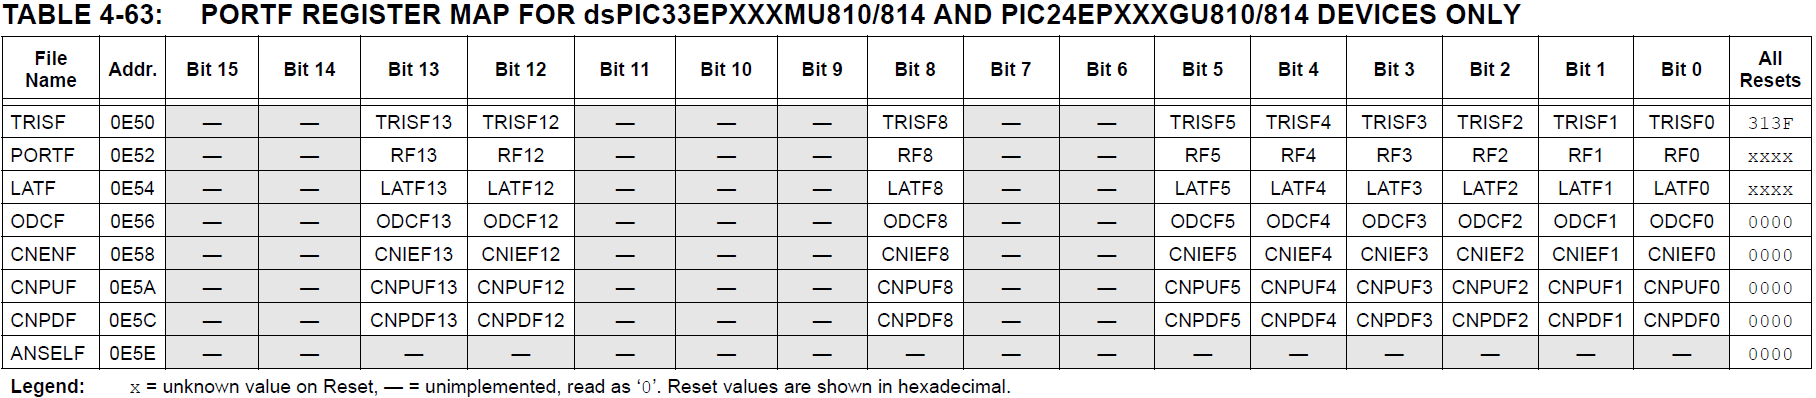
\includegraphics[width=\textwidth]{Images/PORTF}
%	\caption[PORTF Register Map]{PORTF Register Map}
%	\label{image:PORTF}
%\end{figure}
%
%\begin{figure}[!h]
%	\centering
%	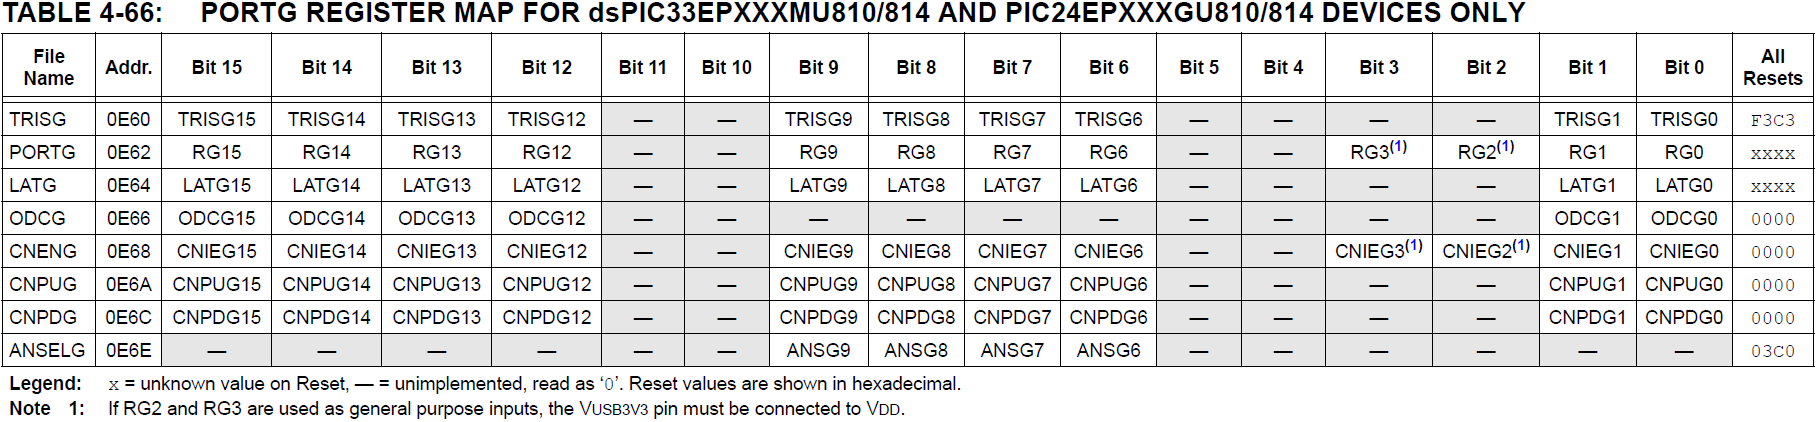
\includegraphics[width=\textwidth]{Images/PORTG}
%	\caption[PORTG Register Map]{PORTG Register Map}
%	\label{image:PORTG}
%\end{figure}

\begin{figure}[!h]
	\centering
	\includegraphics[width=\textwidth]{Images/page207}
	\caption[I/O Ports]{I/O Ports -Datenblatt S.207}
	\label{image:page207}
\end{figure}

\begin{figure}[!h]
	\centering
	\includegraphics[width=\textwidth]{Images/page208}
	\caption[Block Diagramm I/O Ports]{Block Diagramm I/O Ports -Datenblatt S.208}
	\label{image:page208}
\end{figure}	

\begin{figure}[!h]
	\centering
	\includegraphics[width=\textwidth]{Images/page209}
	\caption[I/O Ports]{I/O Ports -Datenblatt S.209}
	\label{image:page209}
\end{figure}

\begin{figure}[!h]
	\centering
	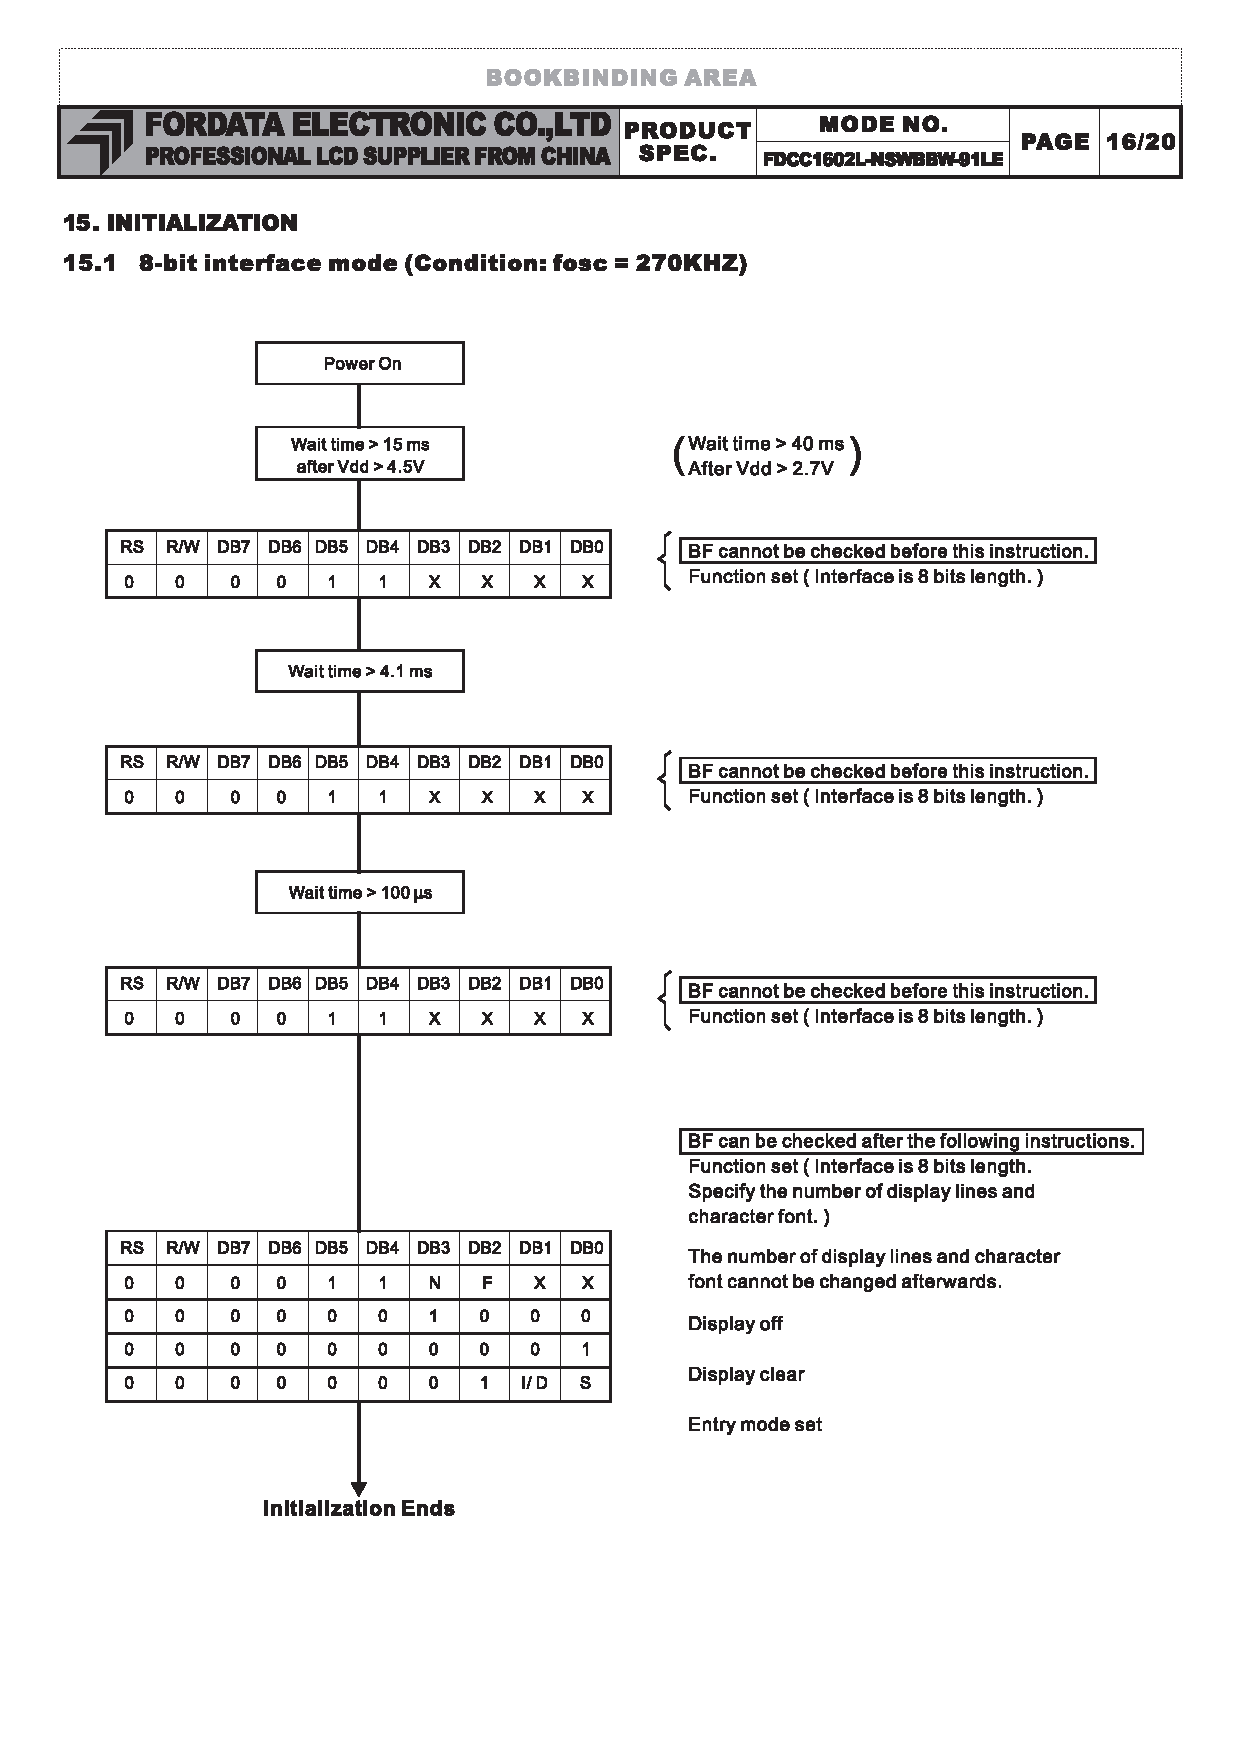
\includegraphics[width=\textwidth]{Images/InitalizationLCD8Bit}
	\caption{LCD Controller Initalization Sequenz}
	\label{image:lcdinit}
\end{figure}


\begin{lstlisting}[frame=htrbl, caption={Initalisierungssequenz des LCD-Controllers}, label={lst:lcdinit}]
void initMyLCD()
{
// 15mS delay after Vdd reaches nnVdc before proceeding with LCD initialization
// not always required and is based on system Vdd rise rate
uint16_t ui16I=0;
while(ui16I++<0xFFFF)Nop();

/* set initial states for the data and control pins */
DATA &= 0xFF00; //set RE0-RE7 low
RW = 0;                         // R/W state set low
RS = 0;                         // RS state set low
E = 0;                          // E state set low

/* set data and control pins to outputs */
TRISE &= 0xFF00;                //set RE0-RE7 to output
RW_TRIS = 0;                    // RW pin set as output
RS_TRIS = 0;                    // RS pin set as output
E_TRIS = 0;                     // E pin set as output

/* 1st LCD initialization sequence */
DATA &= 0xFF00;                 //set RE0-RE7 low
DATA |= 0x0038;                 //set lcd type: 8-bit,2lines,5x7
clockLCDenable();               // toggle E signal
ui16I=0; while(ui16I++<23256)Nop(); //5ms Delay

// 2nd LCD initialization sequence
DATA &= 0xFF00;
DATA |= 0x0038;
clockLCDenable(); 				// toggle Enable signal
ui16I=0; while(ui16I++<4651)Nop(); //200us Delay

// 3rd LCD initialization sequence
DATA &= 0xFF00;
DATA |= 0x0038;
clockLCDenable();
ui16I=0; while(ui16I++<4651)Nop(); //200us Delay

sendCommandLCD( 0x38 );         // function set 8bit, 2lines
sendCommandLCD( 0x0C );         // Display on control, cursor blink off (0x0C), cursor off
sendCommandLCD( 0x06 );         // entry mode set (0x06), increment cursor, no shift 
}
\end{lstlisting}
\newpage

\newpage
\begin{lstlisting}[frame=htrbl, caption={Funktionsprototypen edaPIC33LCD-Library}, label={lst:lcdlib}]
extern char ShadowString[32]; 

void initMyLCD();

void clockLCDenable();

void putcLCD(char c);

void putsLCD(char* pData);

void sendCommandLCD(uint8_t ui8data);

void sendCommandLCDNonBlocking(uint8_t ui8data);

void writeDataLCD(uint8_t ui8data);

void writeDataLCDNonBlocking(uint8_t ui8data);

void setDDRAMAddressLCD(uint8_t ui8address);

uint8_t readBusyFlagLCD();

void putncLCD(char* pData, uint8_t ui8n);

void SendDataToLCD();

void clearLCDStorage();

void SendDataToLCD();

void setLineLCD(const char* pStr, uint8_t ui8Line);

void setLCDLine1(const char* pString);

void setLCDLine2(const char* pString);

\end{lstlisting}
\newpage

\newpage



\end{document}